\newpage
\section{Implémentation}
\subsection{Menu principal}
Sur ce menu principal, nous pouvons voir cinq boutons. 
\begin{itemize}
	\item un bouton "play!" permettant d'accéder au menu jouer
	\item un bouton "settings" permettant d'accéder au menu paramètre
	\item un bouton "leave the game" permettant de quitter le jeu une fois que le joueur à confirmer son choix de 
		fermer le jeu.
	\item un bouton "admin panel" permettant d'accéder au menu d'administration une fois le login réussi.
	\item et enfin un boutton " credits" permettant de voir les crédits du jeu.
\end{itemize}

\begin{figure}[h]
	\centering
	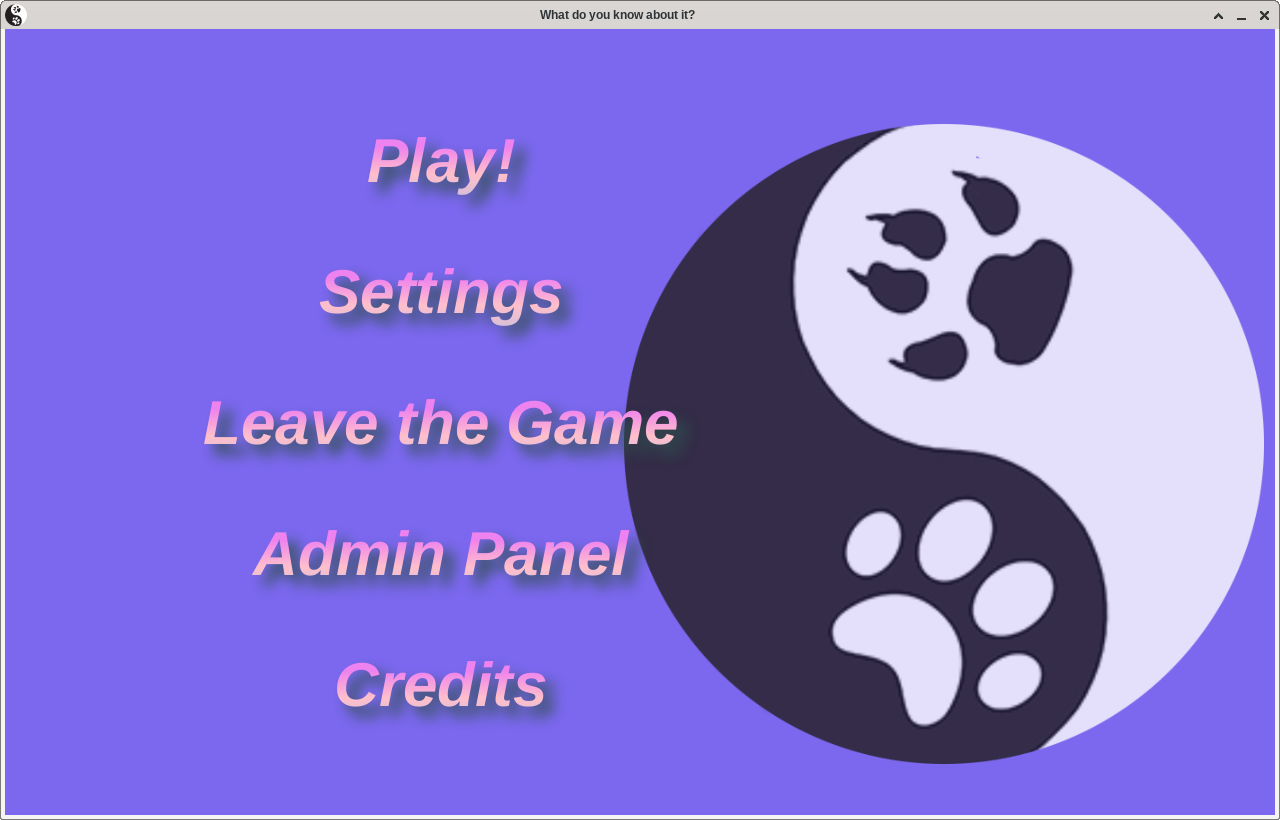
\includegraphics[width=\textwidth]{jeu_main_menu.png}
	\caption{Menu principale du jeu}
	\label{fig:jeu_main_menu}
\end{figure}

\newpage
\subsection{Règle et menu jouer}
Après avoir appuyer sur "Play!", vous arrivez à une fenêtre expliquant les règles du jeu ( celle-ci n'est 
visible que la première fois qu'on appuie sur le boutton "Play!" par lancement de l'application). On accède 
au menu jouer, cette interface possède trois boutons. 
\begin{itemize}
	\item le bouton "Single Player" permettant d'atteindre après avoir mis un pseudo au menu jeu.
	\item le bouton "Multiplayer" permet de parvenir au menu multi joueurs.
	\item le bouton "Return" permet bien evidemment de retourner au menu précédant.
\end{itemize}

\begin{figure}[h]
	\centering
	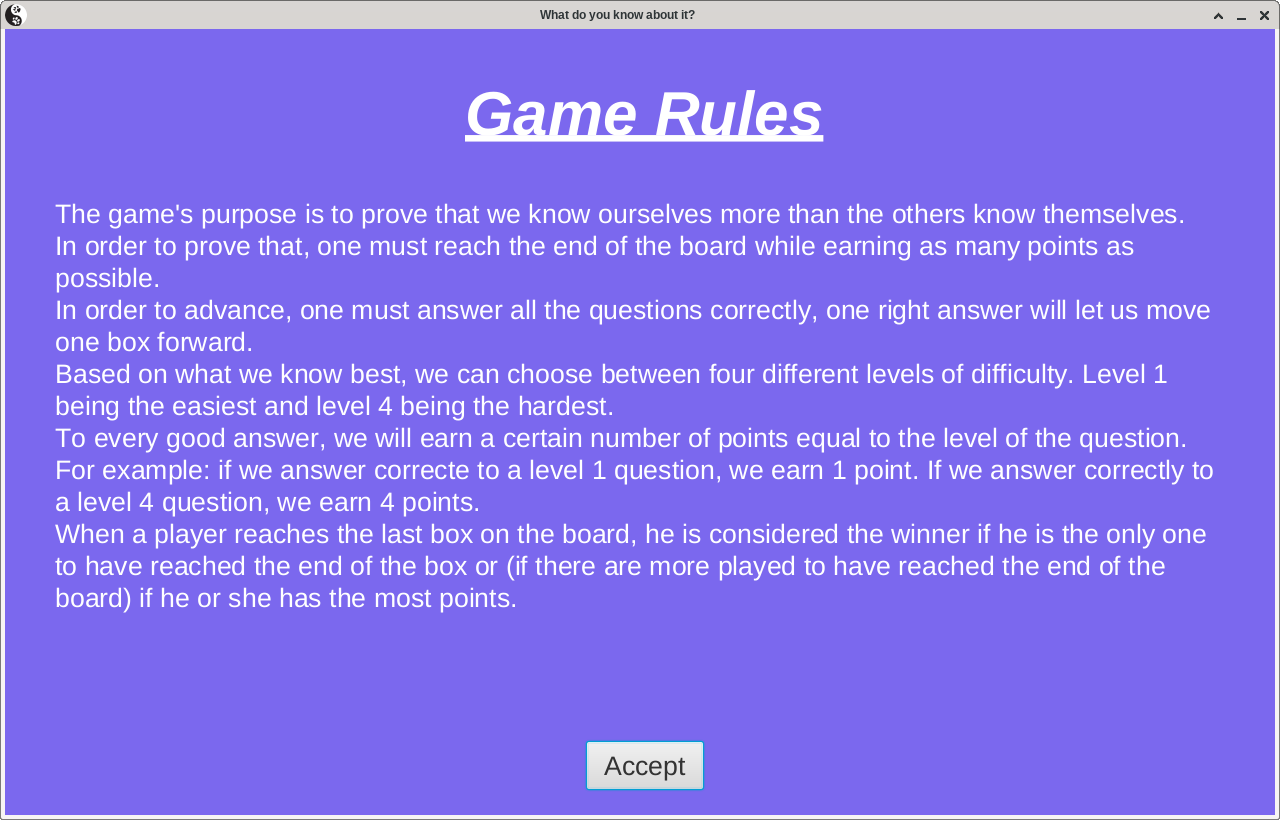
\includegraphics[width=\textwidth]{rule.png}
	\caption{Règle du jeu}
	\label{fig:regle_du_jeu}
\end{figure}

\newpage
\begin{figure}[h]
	\centering
	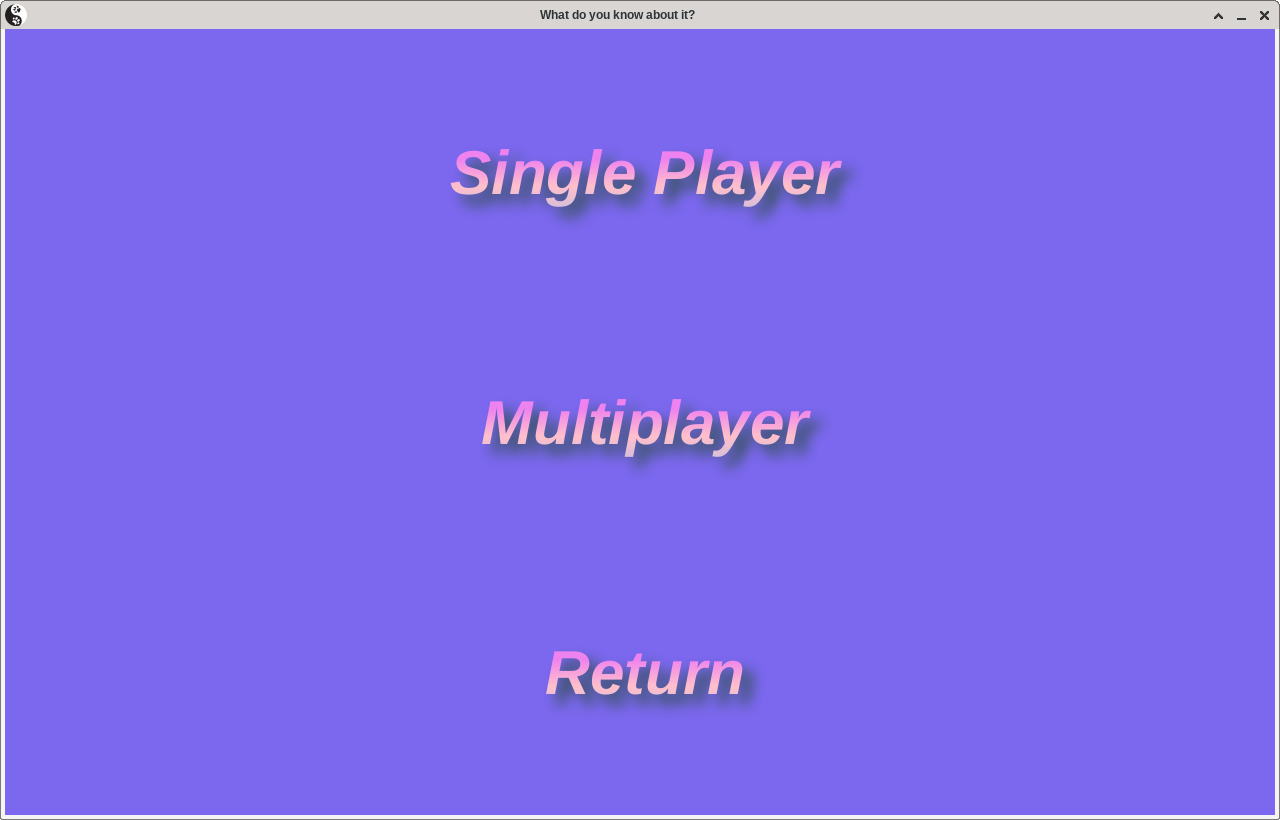
\includegraphics[width=\textwidth]{menujouer.png}
	\caption{menu jouer}
	\label{fig:menu_jouer}
\end{figure}

\newpage
\subsection{Menu jeu}
Menu accessible uniquement en partie solo, ce menu est composé de trois boutons 
\begin{itemize}
	\item Le bouton "New Game" permet de lancer une nouvelle partie.
	\item Le bouton "Load Game" permet de récuperer un deck (fichier json) pour l'utiliser durant la partie.
	\item Le bouton "Return" permet de retourner au menu précédant.
\end{itemize}

\begin{figure}[h]
	\centering
	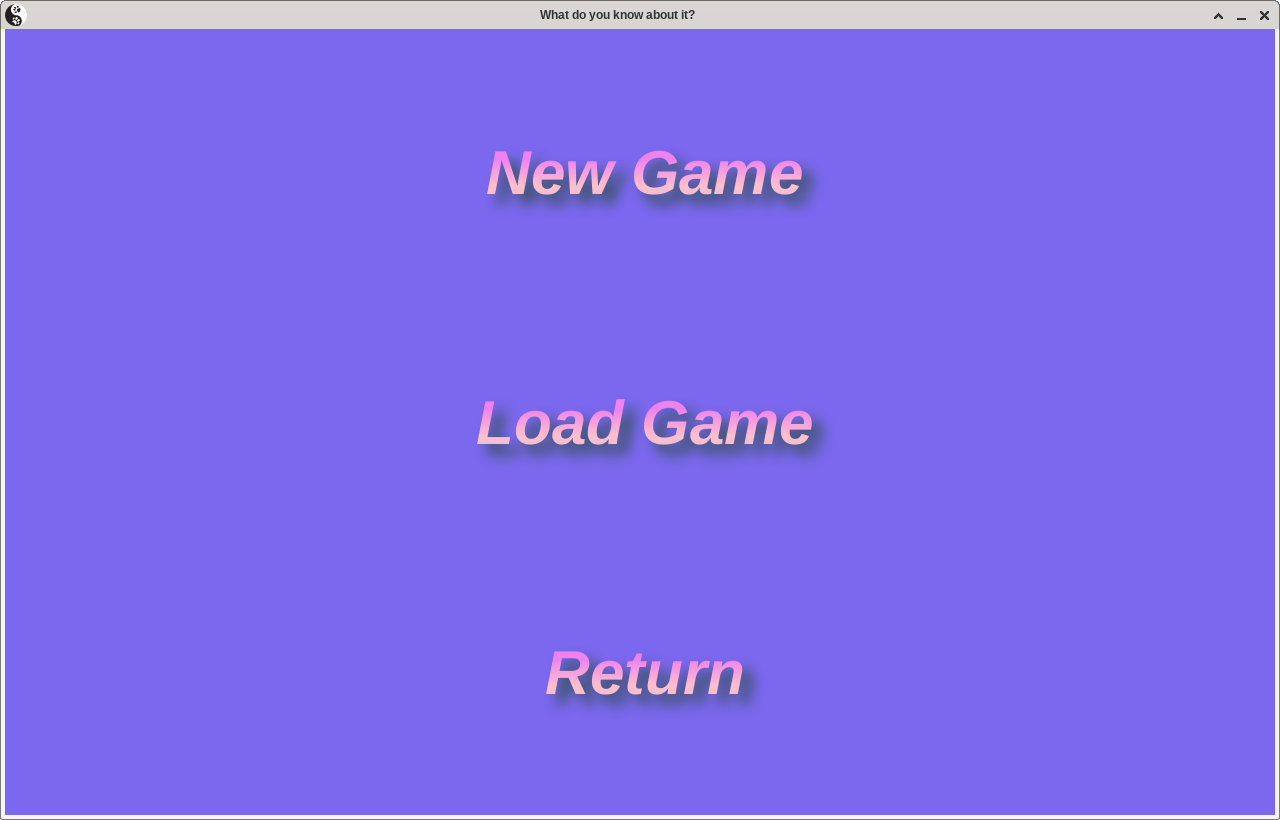
\includegraphics[width=\textwidth]{menujeu.png}
	\caption{menu jeu}
	\label{fig:menu_jeu}
\end{figure}

\newpage
\subsection{Menu multi joueurs}
Dans ce menu, se trouve toute les options disponibles pour les parties multijoueurs. Ce menu est également 
composé de trois boutons.
\begin{itemize}
	\item Un bouton "Local" permet d'accéder à un multi local, il faudra ensuite renseigner le nombre de joueurs
		ainsi que le pseudo de chaque joueur et ensuite appuyer sur "New Game" pour lancer la partie.
	\item Un bouton "Online" permettant d'arriver au menu multijoueur en ligne avec des options propre à se 
		mode de jeu.
	\item le bouton "Return" permet de retourner au menu précédant.
\end{itemize} 

\begin{figure}[h]
	\centering
	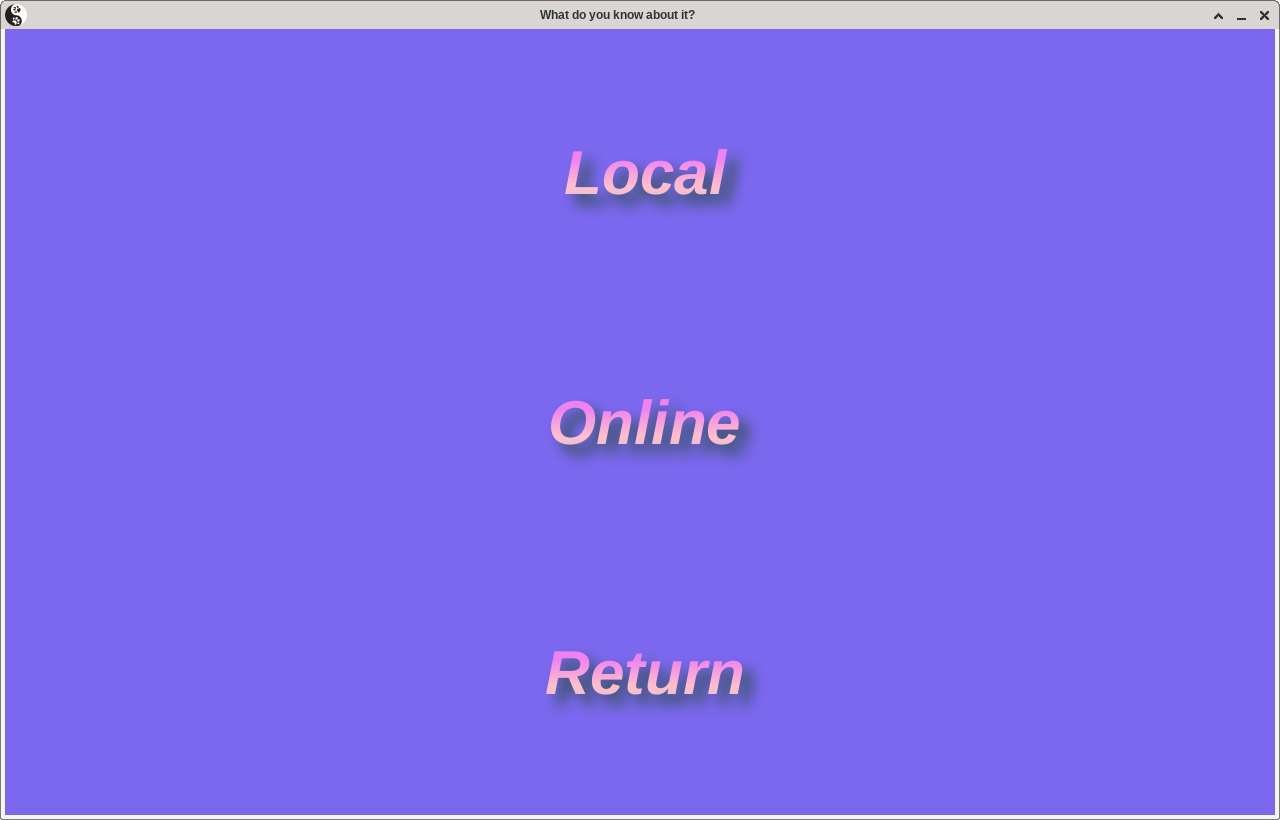
\includegraphics[width=\textwidth]{menumulti.png}
	\caption{menu multi joueurs}
	\label{fig:menu_multi_joueurs}
\end{figure}

\newpage
\subsection{Menu multi joueur en ligne}
Dans ce menu nous retrouverons les options pour le multi en ligne. Ce menu est composé de trois boutons.
\begin{itemize}
	\item Le bouton "Host" permettant d'héberger le jeux.
	\item Le bouton "Join" nous offre la possibilité de rejoindre un joueur hôte. Pour ce faire, après avoir 
		sélectionné cette option, il sera nécessaire de renseigner dans une boite de dialogue  un nom 
		d'utilisateur ainsi que l'adresse IP du joueur hôte.
	\item le bouton "Return" permet de retourner au menu précédant.
\end{itemize}

\begin{figure}[h]
	\centering
	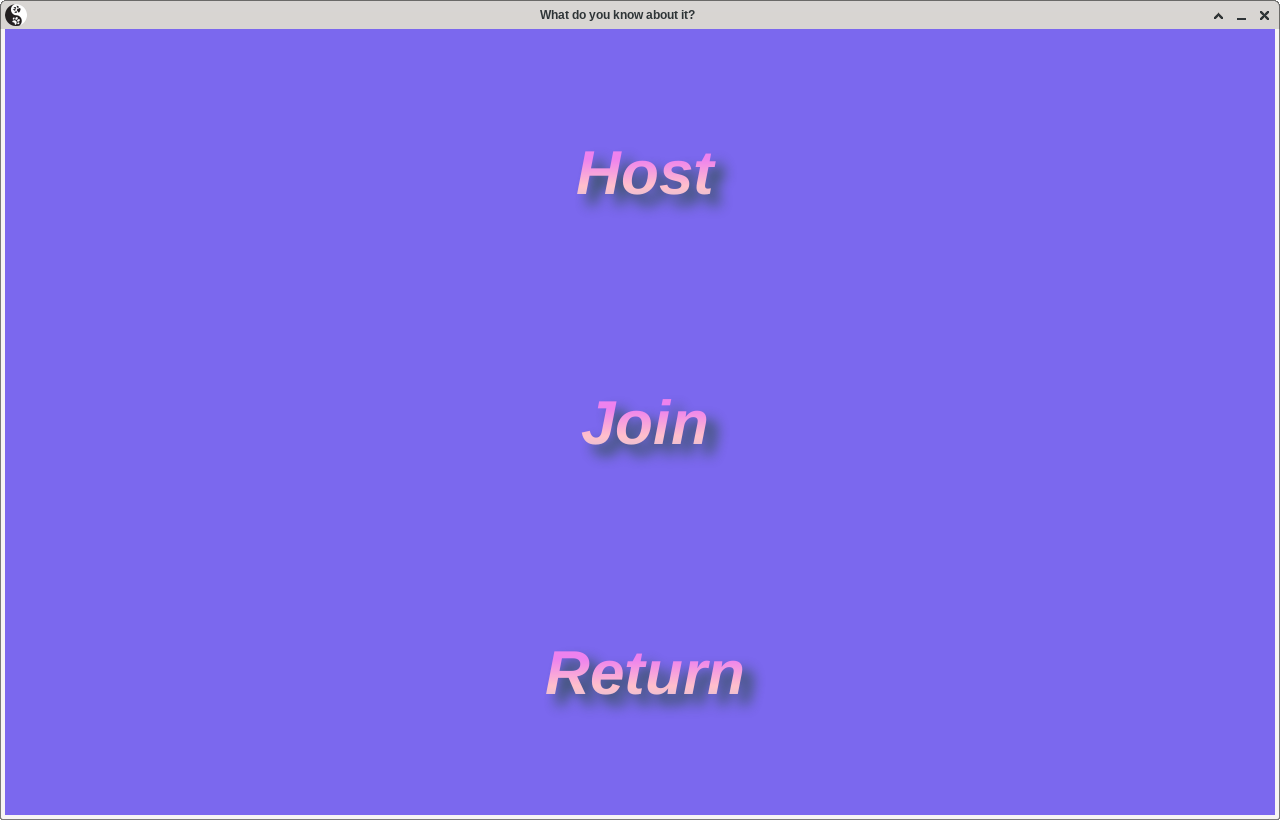
\includegraphics[width=\textwidth]{menuonline.png}
	\caption{menu multi joueur en ligne}
	\label{fig:menu_multi_en_ligne}
\end{figure}

\newpage
\subsection{Menu paramètre}
Ici vous retrouverez tous les options de notre application. Commençons par la barre de volume permettant de gérer 
le volume du son. Cette barre est accompagné d'un bouton "Mute" permettant de complètement mettre le son en 
sourdine. Ensuite ce trouve une textfield permettant de modifier le chrono du jeu. Pour selectionner une langue,
cela se fait depuis une liste déroulante. Les langues disponible sont l'anglais, le français, l'italien et le 
japonais. Vient ensuite une deuxième liste déroulante qui permet cette fois-ci de modifier la taille de la fênetre. Les taille disponible sont 1280x800 et 1440x900. Il est également possible de mettre le jeu en mode plein écran, pour ce faire, il faut cocher l'option "Maximize window".

\begin{figure}[h]
	\centering
	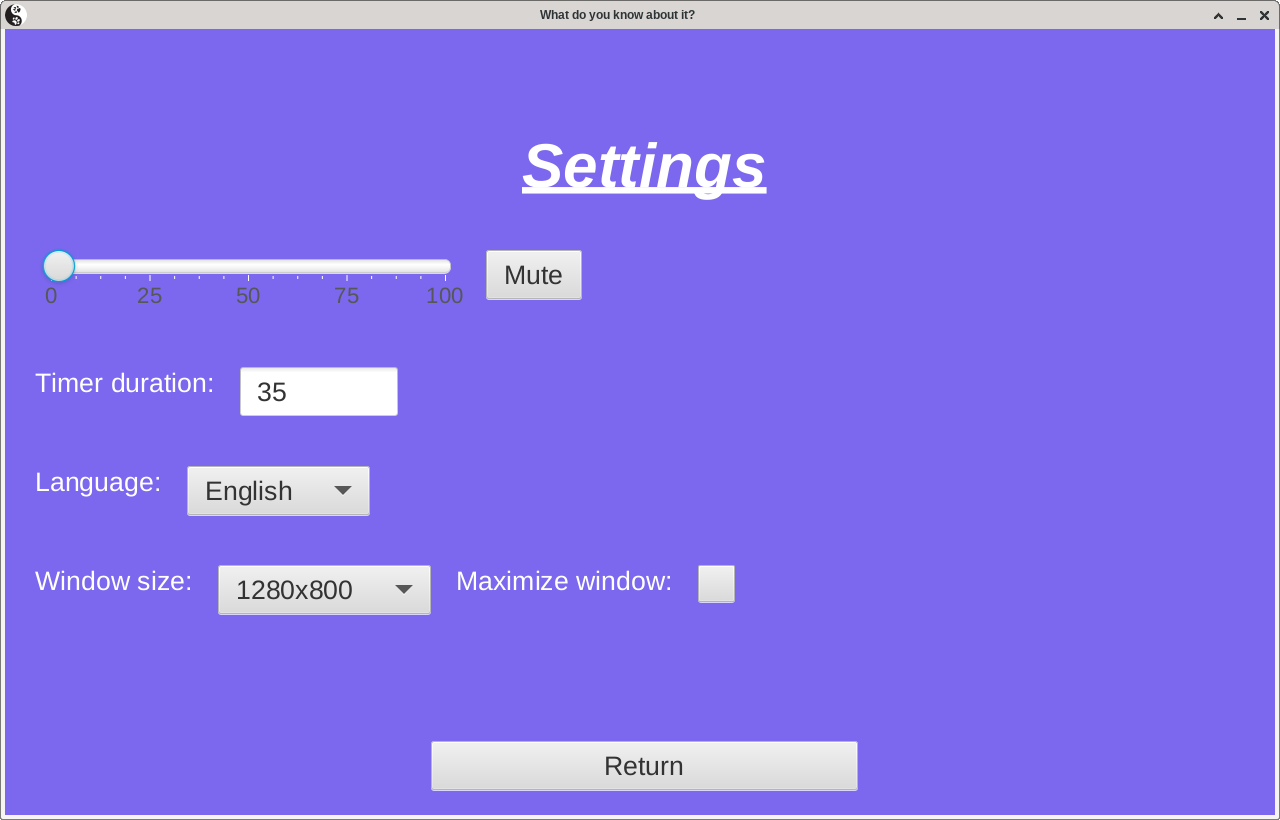
\includegraphics[width=\textwidth]{setting.png}
	\caption{menu paramètre}
	\label{fig:menu_setting}
\end{figure}

\newpage
\subsection{Menu d'administration}
Après avoir cliqué sur le bouton "Admin Panel" du menu principal et vous êtes correctement connecté en tant 
qu'administrateur, vous accéderez au menu administrateur. ce menu est composé de cinq boutons.
\begin{itemize}
	\item Le bouton "Add a new card" permet d'arriver à une nouvelle interface permettant de créer une nouvelle carte.
	\item Le bouton "List of cards" permet d'accèder au tableau de toutes les cartes du deck. Il est également possible de modifier une carte depuis ce tableau
	\item Le bouton "Import a new deck" permet d'importer un nouveau deck pour le jeu. Ce bouton ouvre un explorateur de fichier afin de pouvoir trouver la cible à importer.
	\item Le bouton "Export the current deck" permet d'exporter le deck actuellement utiliser par le jeu. Ce bouton ouvre également un explorateur de fichier afin de pouvoir nommer et placer où on le désire le deck.
	\item le bouton "Return" permet de retourner au menu précédant.
\end{itemize}

\begin{figure}[h]
	\centering
	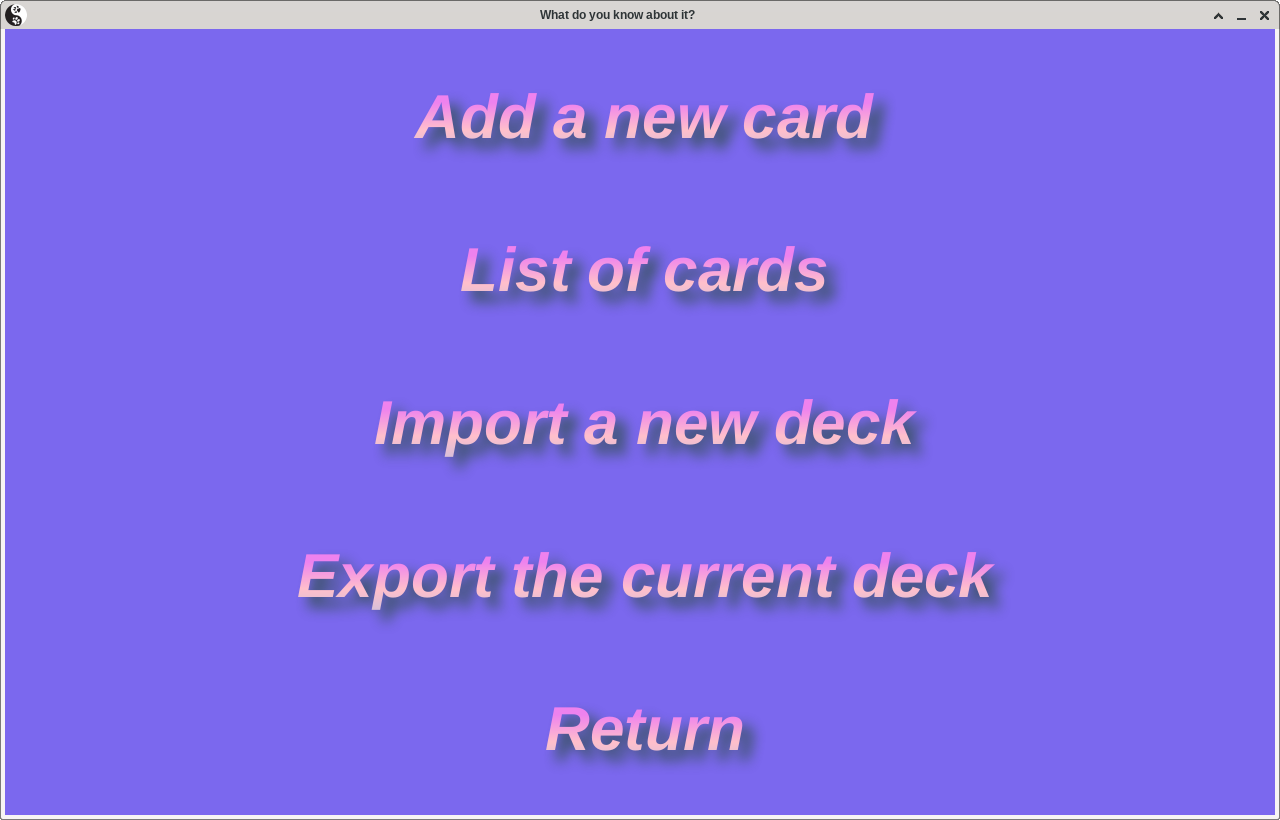
\includegraphics[width=\textwidth]{admin.png}
	\caption{Menu d' administration}
	\label{fig:menu_administration}
\end{figure}

\newpage
\subsection{interface "New Card"}
Cette interface permet d'ajouter une carte au deck. Pour ce faire il faudra d'abord choisir un thème via la 
liste déroulante. Il faudra ensuite renseigner l'auteur, le sujet , les quatres challenge ainsi que les 
quatres réponses. Sachant que le challenge n°1 est le plus facile et donc le challenge 4 est le plus dur.
Le bouton "Add" ajoutera la carte ainsi créé si toute les informations sont bien renseigner. Le bouton "Clean" permet de vider tous les textfields.

\begin{figure}[h]
	\centering
	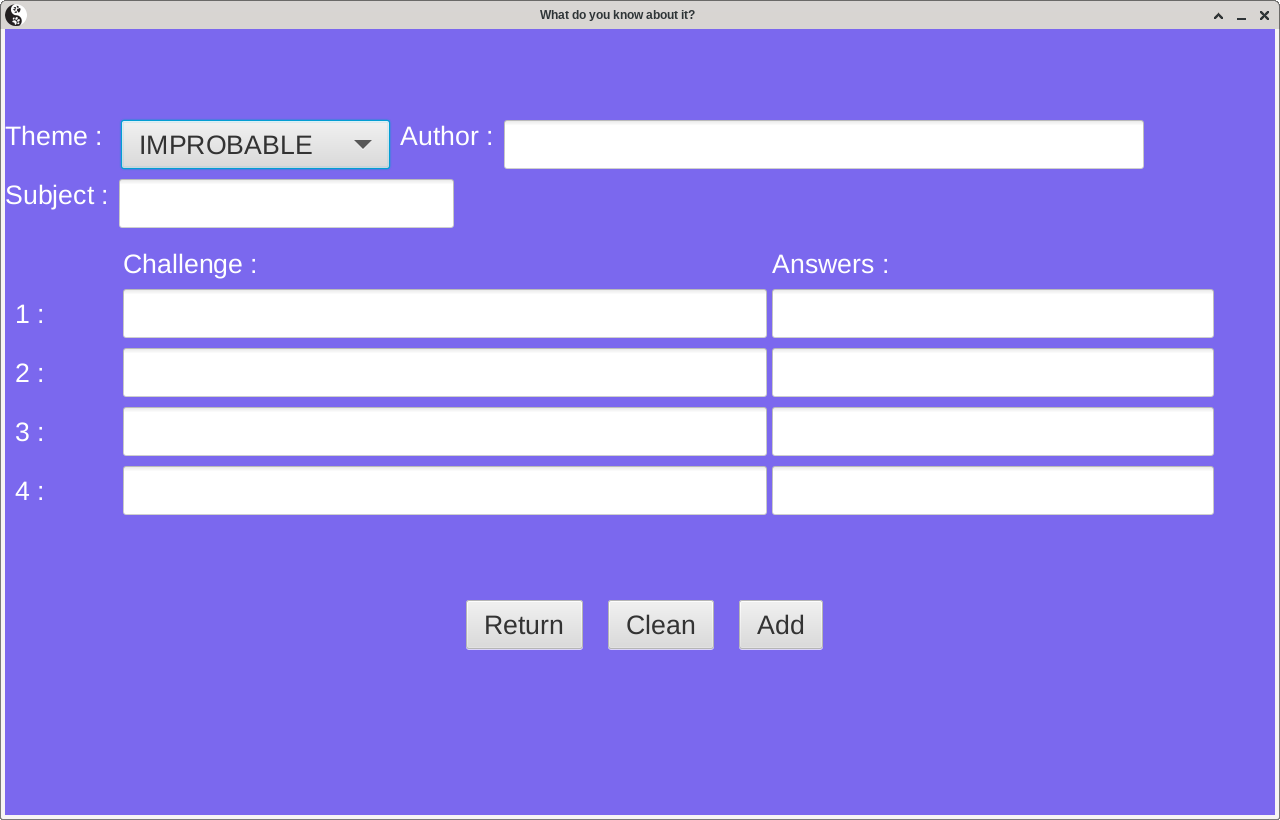
\includegraphics[width=\textwidth]{newcard.png}
	\caption{interface "New card"}
	\label{fig:new_card}
\end{figure}

\newpage
\subsection{Tableau carte}
Cette interface est composé d'un grand tableau de trois colonnes ( auteur, thème et sujet) ainsi que de trois 
boutons. Un bouton "return", un bouton "Reload" permettant de recharger les informations modifier et un bouton 
delete permet à partir d'une sélection de carte de supprimer la carte sélectionné. En double cliquant sur une 
ligne , nous accédons à une interface similaire à "Menu d'administration" si ce n'est que toutes les 
textfields sont déjà rempli. Il ne reste plus qu'à faire les modifications puis appuyer sur" Modify" puis sur "
reload" et toutes les informations ont été mises à jour.

\begin{figure}[h]
	\centering
	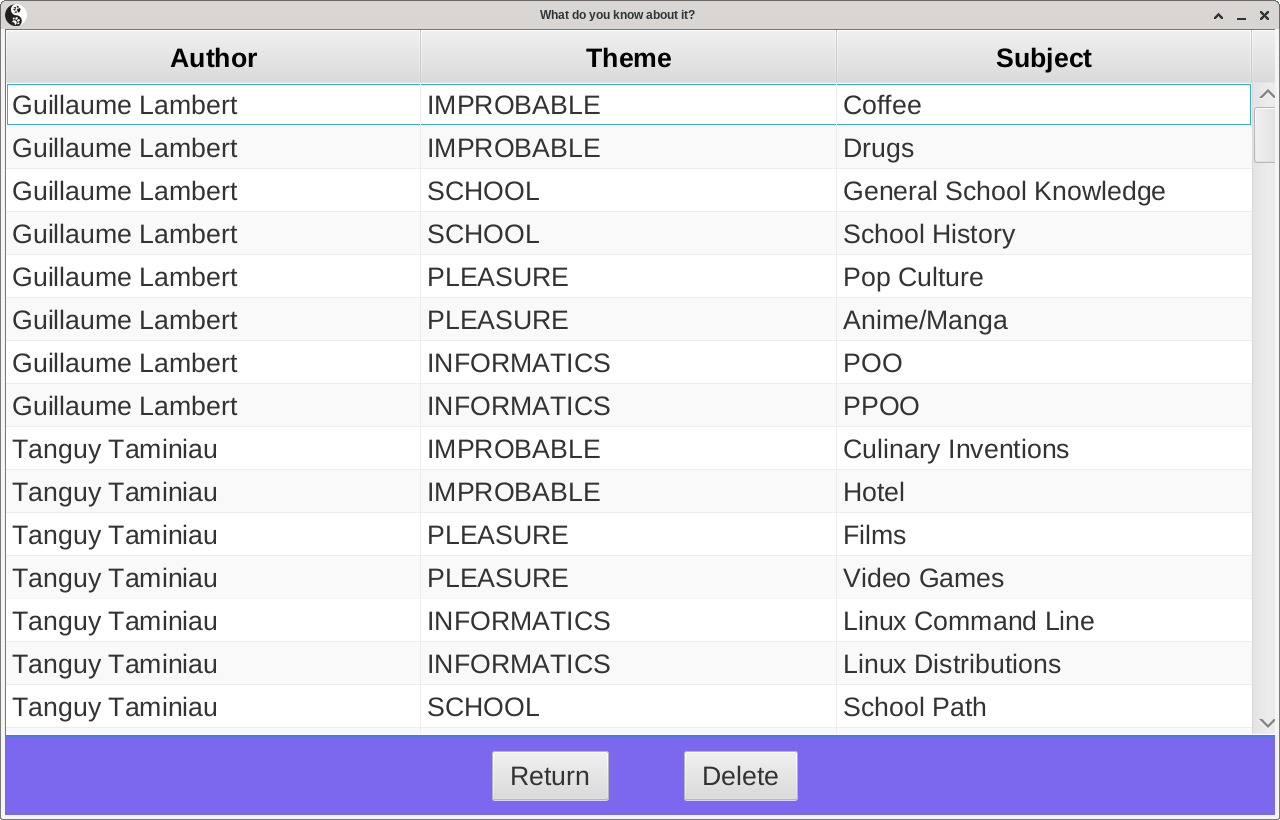
\includegraphics[width=\textwidth]{tablecard.png}
	\caption{Tableau carte}
	\label{fig:tablecard}
\end{figure}
